Other than the definition under definitions, the slides also contains this definition, attributed to Jakob Nielsen:
\begin{description}
	\item[Learnability:] How easy it is for users to accomplish basic tasks the first time they encounter the design?
	\item[Efficiency:] Once users have learned the design, how quickly can they perform the tasks?
	\item[Memorability:] When users return to the design after a period of not using it, how easily can they reestablish proficiency?
	\item[Errors:] How many errors do users make, how severe are these errors, and how easily can they recover from the errors?
	\item[Saticfation] How pleasant is it to use the design?
\end{description}

\textbf{How do we evaluate usability}
\begin{itemize}
	\item Inquiry - \textit{We try to understand users}
	\item Testing - \textit{Users test product designs}
	\item Inspection - \textit{Testing of a design by an expert}
\end{itemize}

\textbf{Usability Testing}
\begin{itemize}
	\item Purpose
	\begin{itemize}
		\item Identifying usability problems in a system
		\item Starting point for refinements of design
	\end{itemize}
	\item Outcome
	\begin{itemize}
		\item A ranked list of usability problems
		\item Knowledge about what works well
	\end{itemize}
	\item How
	\begin{itemize}
		\item Representative users interact with design
		\item Task solving and/or ''thinking-aloud''
		\item Produces a ranked list of usability problems 
	\end{itemize}	
	\item Pros
	\begin{itemize}
		\item Identifies problems very precisely
		\item Gives first-hand insight into use
	\end{itemize}
	\item Cons
	\begin{itemize}
		\item Test situation can be unnatural
		\item Difficult and very time consuming
	\end{itemize}
\end{itemize}

\textbf{When to test}\\
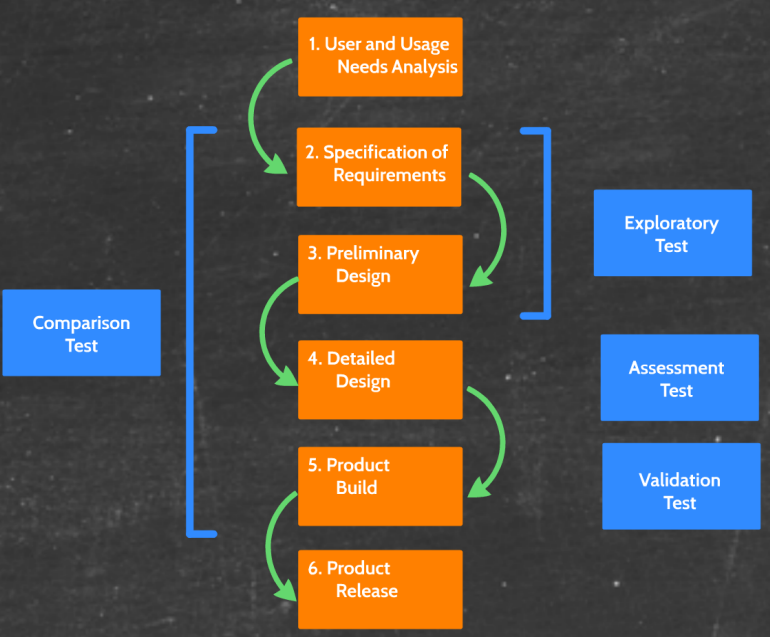
\includegraphics[width=\linewidth]{evaluation-when-to-test}\\

\textbf{Lab vs. field test}
\begin{itemize}
	\item Lab strengths
	\begin{itemize}
		\item The least obtrusive way to collect data
		\item Allows communication ''behind the scene''
		\item Allows many observers
		\item High replicability and control
		\item Demand characteristics
	\end{itemize}
	\item Lab weaknesses
	\begin{itemize}
		\item Somewhat ''sterile'' environment
		\item Test participants may feel like ''lab monkeys''
		\item Questionable realism (ecological validity)
	\end{itemize}
\end{itemize}
\pagebreak
\textbf{Activities in Usability Testing}\\
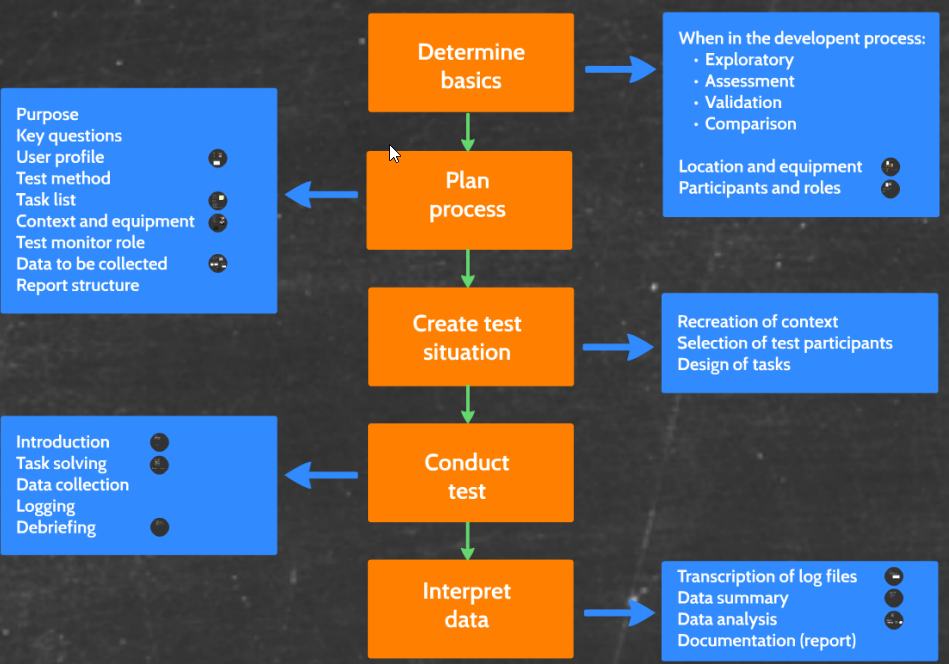
\includegraphics[width=\linewidth]{usability-testing-activities}
\begin{itemize}
	\item Determine basics
	\begin{itemize}
		\item When in the development process
		\begin{itemize}
			\item Exploratory
			\item Assessment
			\item Validation
			\item Comparison
		\end{itemize}
		\item Location and equipment
		\item Participants and roles
	\end{itemize}
	\item Plan process
	\begin{itemize}
		\item Purpose
		\item Key questions
		\item User profile
		\begin{itemize}
			\item Test participants, see figure \ref{fig:usability-test-number-of-tests}
			\begin{itemize}
				\item Representative for the user group
				\begin{itemize}
					\item Demographics
					\item Experience
				\end{itemize}
				\item Number of test subjects
				\begin{itemize}
					\item Generalizability
					\item Quantitative conclusions
					\item Statistics
				\end{itemize}
				\item Using fellow students
				\begin{itemize}
					\item Problematic...
					\item Motivation
					\item Demographics and experience
				\end{itemize}
			\end{itemize}
		\end{itemize}
		\item Test method
		\item Task list
		\begin{itemize}
			\item Deciding on the Tasks
			\begin{itemize}
				\item What are the basic tasks that representative users do with the system?
				\item Is the whole system part of the evaluation?
				\item Can we create a crystal clear task description?
				\item How long does it take to solve the tasks?
				\item Some useful rules for defining tasks
				\begin{itemize}
					\item Make the Tasks Realistic
					\item Make the Tasks Actionable
					\item Avoid Clues and Describing the Steps
				\end{itemize}
				\item Good tasks
				\begin{itemize}
					\item Represent real use of the system
					\item Describe the end result
					\item Motivate (why should they be solved?)
					\item Include relevant data (e.g. names)
					\item Group smaller sub-tasks together
				\end{itemize}
				\item Typical problems
				\begin{itemize}
					\item Vague, unclear or general
					\item Provides too much help
					\item Contain jargon and unfamiliar terms
					\item Forces the user into a specified sequence
				\end{itemize}
			\end{itemize}
		\end{itemize}
		\item Context and equipment
		\begin{itemize}
			\item Context of use
			\begin{itemize}
				\item Where is the design/system used?
				\begin{itemize}
					\item Physical environment?
					\item Social context?
				\end{itemize}
				\item Who uses the design?
				\begin{itemize}
					\item User profiles
				\end{itemize}
				\item Why is the design used?
				\begin{itemize}
					\item What do people use it for?
					\item Work? Leisure? Other activities?
				\end{itemize}
				\item How is the design used?
				\begin{itemize}
					\item Typical interactions
					\item Relevant and realistic data
				\end{itemize}
			\end{itemize}
		\end{itemize}
		\item Test monitor role
		\item Data to be collected
		\begin{itemize}
			\item Deciding on what to measure and how
			\begin{itemize}
				\item Are all the components of usability relevant?
				\item How will we collect data?
				\item What are we going to measure?
				\item Think aloud?
			\end{itemize}
			\item Usability metrics
			\begin{itemize}
				\item Objective metrics
				\begin{itemize}
					\item Effectiveness - how many tasks were completed
					\item efficiency - how fast were they completed
				\end{itemize}
				\item Subjective metrics
				\begin{itemize}
					\item Interview data
					\item Questionnaires
				\end{itemize}
			\end{itemize}
			\item Video recordings
			\begin{itemize}
				\item The whole scene?
				\item The screen?
				\item The surroundings?
			\end{itemize}
		\end{itemize}
		\item Report structure
	\end{itemize}
	\item Create test situation
	\item Conduct test
	\begin{itemize}
		\item Introduction
		\begin{itemize}
			\item Instructions about the test
			\item Consent form
			\item Questionnaire (demographics)
		\end{itemize}
		\item Task solving
		\begin{itemize}
			\item Test subject ''thinks-aloud''
			\item Test monitor facilitates. May provide help
			\begin{itemize}
				\item Important characteristics
				\begin{itemize}
					\item Solid knowledge about usability
					\item Fast learner
					\item Can establish good relations to subjects
					\item Good memory
					\item Good at listening
					\item Good at communication
					\item Can handle uncertainty
					\item Flexible and capable of improvising
					\item Can stay alert for a long time
					\item Can maintain an overview
				\end{itemize}
				\item Typical problem
				\begin{itemize}
					\item Controlling rather than supporting
					\item Too focused on data collection
					\item Sticks too close to test plan
					\item Appears better knowing
					\item Does not establish good relations
					\item Jumps to conclusions
				\end{itemize}
			\end{itemize}
			\item Test session is recorded observer takes notes and creates log file
		\end{itemize}
		\item Data collection
		\item Logging
		\item Debriefing
		\begin{itemize}
			\item Done immediately after the evaluation session
			\item Can include
			\begin{itemize}
				\item Filling out a questionnaire with opinions
				\item An interview: explaining particular events in the evaluation
				\item Critiquing the interaction design
				\item User suggesting solutions and design ideas
			\end{itemize}
			\item Allow enough time for discussion
		\end{itemize}
	\end{itemize}
	\item Interpret data
	\begin{itemize}
		\item Transcription of log files
		\begin{itemize}
			\item The log file is an important document in the analysis, see figure \ref{fig:usability-test-log-file}
			\begin{itemize}
				\item Simplified transcription of the evaluation
				\item Captures the user interaction in textual form
				\item Provides overview and ''filtered detail''
				\item Relation between time, event, and usability problems
				\item specialized tools exists - but at table in Word will do.
				\item Can be created ''live'' during tests, and finished from video recordings
			\end{itemize}
		\end{itemize}
		\item Data summary
		\begin{itemize}
			\item Summarize the number of usability problems, total and in categories.
			\item How many of the problems were ''unique''
		\end{itemize}
		\item Data analysis
		\begin{itemize}
			\item What is a usability problem?
			\begin{itemize}
				\item For user-based evaluations
				\begin{itemize}
					\item \textit{A problem experienced by a specific user while interacting with a specific system}
					\item The user...
					\begin{itemize}
						\item is delayed or prevented in completing a task
						\item feels frustrated
						\item makes mistakes
						\item misses important information
						\item stops talking
						\item is confused or surprised
						\item changes strategy or approach
						\item asks for help
						\item makes negative comments
					\end{itemize}
				\end{itemize}
				\item For expert-based evaluations
				\begin{itemize}
					\item \textit{A \textbf{potential} problem identified by a specific expert to be in conflict with a specific heuristic or guideline}
				\end{itemize}
			\end{itemize}
			\item The problem list, see figure \ref{fig:usability-test-problem-list}
			\begin{itemize}
				\item The problem list is the primary outcome from an evaluation
				\item A ranked, and numbered, list of usability problems
				\item Indicates how many users experienced the problem (and who)
				\item Indicates where in the system the problem was experienced
				\item Describes each identified usability problem in detail and with brief examples
				\item The problem/description may fo across several tasks
				\item May be divided into two lists: overview and detail, see figure \ref{fig:usability-test-detail-list}
			\end{itemize}
			\item Categorizing problems
			\begin{itemize}
				\item Typically three categories, see table \ref{tbl:usability-problems-categories}
				\item Critical problem
				\begin{itemize}
					\item Unable to continue
					\item Feels the system behaves strongly irritating
					\item Critical difference between believed and actual state of the system
				\end{itemize}
				\item Catastrophic
				\begin{itemize}
					\item More than one user experience the same critical problem independently
				\end{itemize}
			\end{itemize}
		\end{itemize}
		\item Documentation (report)
	\end{itemize}
\end{itemize}
\begin{figure}
	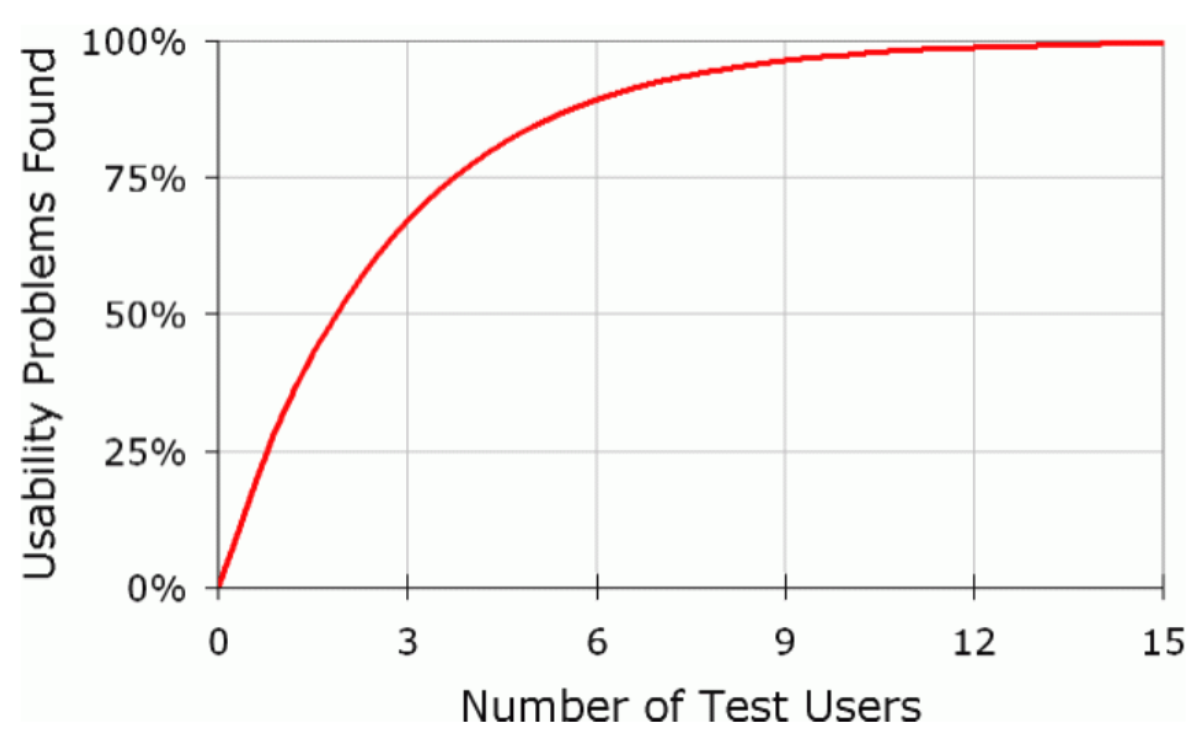
\includegraphics[width=\linewidth]{usability-test-number-of-tests}
	\caption{The number of test persons to find all usability problems}
	\label{fig:usability-test-number-of-tests}
\end{figure}
\begin{figure*}
	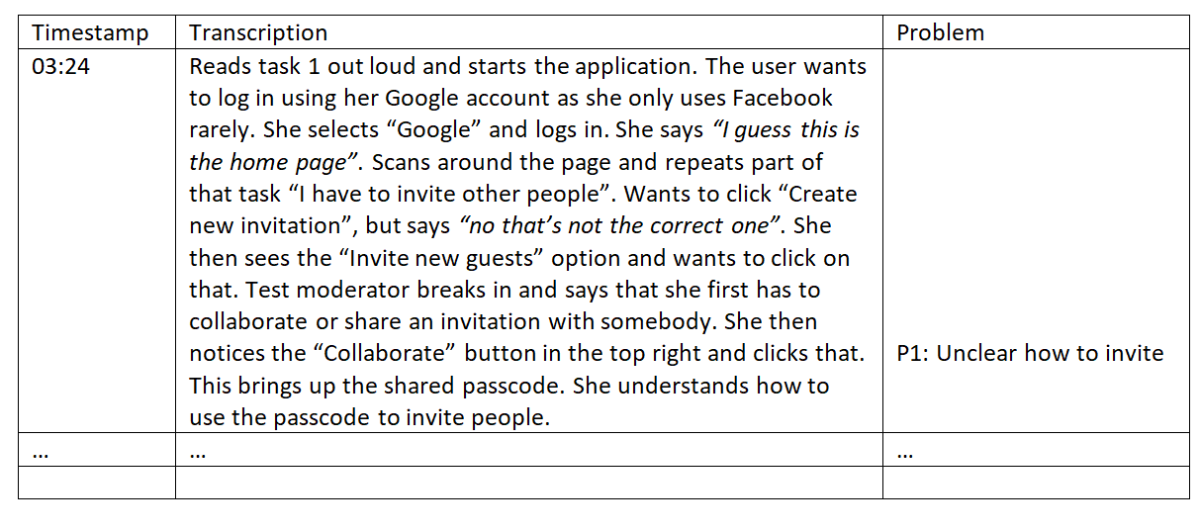
\includegraphics[width=\linewidth]{usability-test-log-file}
	\caption{Usavility test logfile}
	\label{fig:usability-test-log-file}
\end{figure*}
\begin{figure*}
	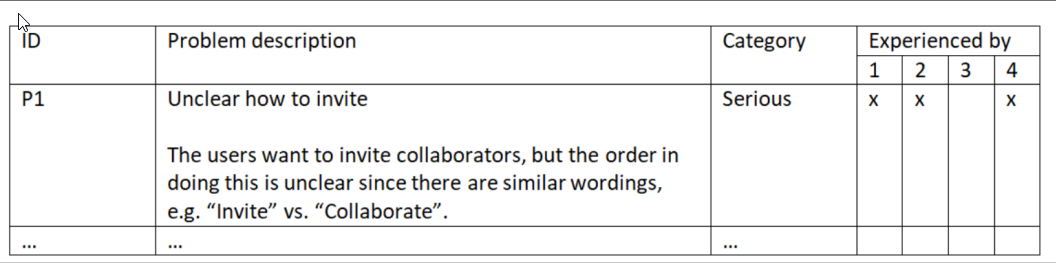
\includegraphics[width=\linewidth]{usability-test-problem-list}
	\caption{Problem list}
	\label{fig:usability-test-problem-list}
\end{figure*}
\begin{figure*}
	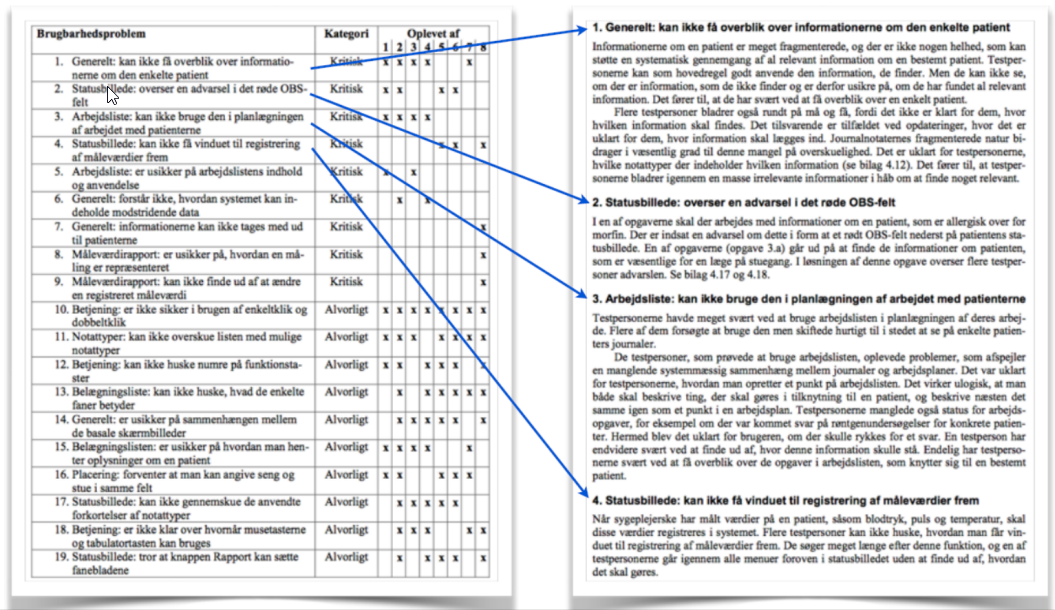
\includegraphics[width=\linewidth]{usability-test-detail-list}
	\caption{Problem list, and detailed list}
	\label{fig:usability-test-detail-list}
\end{figure*}
\begin{table*}
	\centering
	\begin{tabular}{llll}
		\toprule
		 & \textbf{\textit{Delay}} & \textbf{\textit{Irritation}} & \textbf{\textit{Expectation vs. actual}} \\ \midrule
		 \textbf{\textit{Cosmetic}} & $<1$ minute & Low & Small diff.\\
		 \textbf{\textit{Serious}} & Several minutes & Medium & Significant diff.\\
		 \textbf{\textit{Critical}} & Total(user stops) & Strong & Critical diff.\\\bottomrule
	\end{tabular}
	\caption{Usability problem categories and explanations}
	\label{tbl:usability-problems-categories}
\end{table*}
\clearpage
\textbf{Heuristic Inspection}\\
\begin{itemize}
	\item Usability experts inspects a design using a checklist (heuristic)
	\item Scenarios + relevant tasks can structure the process
	\item Produces a ranked list of usability problems
	\item Pros
	\begin{itemize}
		\item Quick and easy to conduct
		\item No users requires
		\item 3-5 inspections finds 70\% of all problems
	\end{itemize}
	\item Cons
	\begin{itemize}
		\item High proportion of ''cosmetic'' problems
		\item ''False'' usability problems
	\end{itemize}
\end{itemize}
\textbf{Usability problems are present when the system is}
\begin{description}
	\item[Unuseful] - You cannot find the documents or functions you need to solve your tasks.
	\item[Difficult to learn] - It takes a long time to learn how to use the system.
	\item[Difficult to remember] - It takes a long time to find elements in the system, which you have used previously.
	\item[Ineffective to use] - It takes a long time to solve certain tasks with the system.
	\item[Unsatisfying to use] - The system does not feel comfortable to use, it is not joyful to work with it.
\end{description}